%
% auth: Mattijs Korpershoek
% mail: <mattijs.korpershoek@gmail.com>
%
\documentclass[compress]{beamer}
%%%%%%%%%%%%%%
%  Packages  %
%%%%%%%%%%%%%%
\usepackage[english]{babel}
\usepackage[T1]{fontenc}
\usepackage{lmodern}
\usepackage{microtype}
\usepackage{multicol}
\usepackage[normalem]{ulem}
\usepackage{soul}
\usepackage{listings}
\usepackage{caption}
\usepackage{textpos} % for textblock
\usepackage{mathtools} % math environment
\usepackage{textcomp}
\usepackage{pgfgantt}
\usepackage{dirtree}

%%%%%%%%%%%%%%%%%%%%%
% Special variables %
%%%%%%%%%%%%%%%%%%%%%
\newcommand{\ImageFolder}{./img}

%%%%%%%%%%%%%%%%%%%%%%%
% Beamer environments %
%%%%%%%%%%%%%%%%%%%%%%%
% sets automatically the current subsection as frame title on your slide
\newenvironment<>{FrameWithSubSection}%
{%
  \begin{frame}%
    \frametitle{\insertsubsectionhead}%
    \par%
  }
  {%
    \par%
  \end{frame}%
}
% the % are at the end of each line because with some text editors,
% the LaTeX compiler may understand the \n as a command caracter.

%%%%%%%%%%%%%%%%%%%%%%
%  Solarized colors  %
%%%%%%%%%%%%%%%%%%%%%%
\definecolor{base03}{HTML}{002B36}
\definecolor{base02}{HTML}{073642}
\definecolor{base01}{HTML}{586E75}
\definecolor{base00}{HTML}{657B83}
\definecolor{base0}{HTML}{839496}
\definecolor{base1}{HTML}{93A1A1}
\definecolor{base2}{HTML}{EEE8D5}
\definecolor{base3}{HTML}{FDF6E3}
\definecolor{yellow}{HTML}{B58900}
\definecolor{orange}{HTML}{CB4B16}
\definecolor{red}{HTML}{DC322F}
\definecolor{magenta}{HTML}{D33682}
\definecolor{violet}{HTML}{6C71C4}
\definecolor{blue}{HTML}{268BD2}
\definecolor{cyan}{HTML}{2AA198}
\definecolor{green}{HTML}{859900}



%%%%%%%%%%%%%%%%%%%%
% caption settings %
%%%%%%%%%%%%%%%%%%%%
\DeclareCaptionFont{captionText}{\color{base1}}
\DeclareCaptionFormat{listing}{\colorbox{base03}{\parbox{0.985\textwidth}{\hspace{15pt}#1#2#3}}}
\captionsetup[lstlisting]{format=listing,labelfont=captionText,textfont=captionText, singlelinecheck=true, margin=0pt, font={sf,footnotesize}}
\DeclareCaptionFormat{figure}{\colorbox{base03}{\parbox{0.985\textwidth}{\hspace{15pt}#1#2#3}}}
\captionsetup[figure]{format=figure,labelfont=captionText,textfont=captionText, singlelinecheck=false, margin=0pt, font={sf,footnotesize}}

\lstdefinelanguage{pfwLang}
{morekeywords={Domain, Conf, Component},
sensitive=false,
morecomment=[l]{\#},
morestring=[b]",
}

\usepackage{inconsolata}
\lstset{
    basicstyle=\ttfamily\footnotesize,
    language=C,
    frame=lines,
    sensitive=true
    tabsize=2,
    breaklines=true,
    showstringspaces=false,
    showspaces=false,
    backgroundcolor=\color{base3},
    keywordstyle=\color{blue},
    commentstyle=\color{base1},
    stringstyle=\color{cyan},
    numberstyle=\color{violet},
    rulecolor=\color{base00},
    morekeywords={pfw, setParameter, getParameter}
}

\lstnewenvironment{code}[1][]%
{
    \noindent
    \minipage{\linewidth}
    \vspace{0.5\baselineskip}
        \lstset{#1}}
{\endminipage}

%%%%%%%%%
% fonts %
%%%%%%%%%
\usefonttheme[onlymath]{serif}
\usepackage{fontspec}
\defaultfontfeatures{Mapping=tex-text}
\setsansfont[Ligatures={Common}]{Futura}

%%%%%%%%%%%%%%%%
% Beamer Theme %
%%%%%%%%%%%%%%%%
%\usetheme{Warsaw}

\useinnertheme{circles}
\useoutertheme{split}

%\usecolortheme[RGB={255,51,0}]{structure} % Paul sabatier red logo color

%\setbeamercolor{alerted text}{fg=orange}
%\setbeamercolor{background canvas}{bg=base3}
%\setbeamercolor{block body alerted}{bg=normal text.bg!90!black}
%\setbeamercolor{block body example}{bg=normal text.bg!90!black}
%\setbeamercolor{block title alerted}{use={normal text,alerted text},fg=alerted text.fg!75!normal text.fg,bg=normal text.bg!75!black}
%\setbeamercolor{block title example}{use={normal text,example text},fg=example text.fg!75!normal text.fg,bg=normal text.bg!75!black}
%\setbeamercolor{fine separation line}{}
%\setbeamercolor{frametitle}{fg=base3}
%\setbeamercolor{item projected}{fg=black}
%\setbeamercolor{normal text}{bg=base2,fg=base02}
%\setbeamercolor{palette sidebar primary}{use=normal text,fg=normal text.fg}
%\setbeamercolor{palette sidebar quaternary}{use=structure,fg=structure.fg}
%\setbeamercolor{palette sidebar secondary}{use=structure,fg=structure.fg}
%\setbeamercolor{palette sidebar tertiary}{use=normal text,fg=normal text.fg}
%\setbeamercolor{section in sidebar}{fg=orange}
%\setbeamercolor{section in sidebar shaded}{fg=grey}
%\setbeamercolor{separation line}{}
\setbeamercolor{sidebar}{bg=blue}
\setbeamercolor{structure}{fg=blue}
%\setbeamercolor{subsection in sidebar}{fg=brown}
%\setbeamercolor{subsection in sidebar shaded}{fg=grey}
%\setbeamercolor{title}{fg=brown}
%\setbeamercolor{titlelike}{fg=brown}
\setbeamercolor{block body}{bg=base2 text.bg!90!base02}
\setbeamercolor{block title}{bg=blue}

\usetheme{Berlin}
\useoutertheme[]{miniframes}

\defbeamertemplate*{footline}{shadow theme}
{%
  \leavevmode%
  \hbox{\begin{beamercolorbox}[wd=.5\paperwidth,ht=2.5ex,dp=1.125ex,leftskip=.3cm plus1fil,rightskip=.3cm]{author in head/foot}%
      \usebeamerfont{author in head/foot}\insertframenumber\,/\,\inserttotalframenumber\hfill\insertshortauthor
    \end{beamercolorbox}%
    \begin{beamercolorbox}[wd=.5\paperwidth,ht=2.5ex,dp=1.125ex,leftskip=.3cm,rightskip=.3cm plus1fil]{title in head/foot}%
      \usebeamerfont{title in head/foot}\insertshorttitle%
  \end{beamercolorbox}}%
  \vskip0pt%
}


%%%%%%%%%%%%
% Document %
%%%%%%%%%%%%
\begin{document}
% inserts at every new section the Overview
%\AtBeginSection[]
%{
%  \frame<beamer>{\begin{multicols}{2}
%      \frametitle{Table of contents}
%      \tableofcontents[currentsection,currentsubsection]
%    \end{multicols}
%  }
%}

%
% auth: Mattijs Korpershoek
% mail: <mattijs.korpershoek@gmail.com>
%

\title{Internship presentation}
\subtitle{Open-sourcing the Parameter-framework}
\author{Mattijs Korpershoek}
\institute{Master CAMSI, Université Paul Sabatier}
\date{05/09/2014}

\begin{frame}
  \maketitle
{
    % include logos only on front page
    \includegraphics[height=1cm]{\ImageFolder/logointel.jpg}\hfill
    \includegraphics[height=1cm]{\ImageFolder/logoupsNew.jpg}
    \hfill \includegraphics[height=1cm]{\ImageFolder/logocelad.jpg}
}
\end{frame}

%
% auth: Mattijs Korpershoek
% mail: <mattijs.korpershoek@gmail.com>
%

\section{Introduction}

\subsection{Introduction}
\begin{FrameWithSubSection}
    \begin{itemize}
        \item Internship of 6 months
        \item Middleware, Android, Open-sourcing
    \end{itemize}
\end{FrameWithSubSection}

\subsection{Table of contents}
% table of contents
\frame<beamer>{\begin{multicols}{2}
        \frametitle{Table of contents}
        \tableofcontents
    \end{multicols}
}

\chapter{Context}\label{chap:context}

\begin{sectionIntro}
    TODO
\end{sectionIntro}

\section{Company}

\subsection{CELAD}
One of its biggest clients in the embedded sector in Toulouse is Intel.
TODO

\subsection{Intel}
Intel is a big company, with multiple divisions.
TODO

\subsection{Audio feature team in Toulouse}
The team I worked with is the audio feature team, in Toulouse.

\section{Android}

\subsection{Global Android architecture}
TODO figure from wikipedia

\subsection{Intel Audio HAL}
HAL, multiple platforms with different architectures.
Scalable, fully configurable, userland.
TODO

\subsection{Parameter-framework}
\label{sec:parameter-framework}
Middleware, gap, no standard.
Internship was around the parameter-framework. Middleware standard. Audio team. Opensourcing.


%
% auth: Mattijs Korpershoek
% mail: <mattijs.korpershoek@gmail.com>
%
\section{Methodology}

\subsection{Time distribution}
\begin{FrameWithSubSection}
\begin{ganttchart}[
        x unit=0.5cm,
        y unit title=.6cm,
        y unit chart=.6cm,
        hgrid=true,
        vgrid={*1{red,  dotted}},
        canvas/.style={fill=base2},
        bar/.style={fill=orange},
        title/.style={fill=base2},
        group/.style={fill=blue, shape=ganttgroup},
        bar height = 0.4,
    ]{1}{24}
    \gantttitlelist{1, ..., 24}{1} \\
    \ganttbar{Arrival, installation}{1}{1} \\
    \ganttgroup{Client deliverable}{4}{20} \\
    \ganttbar{Improving build process}{4}{11} \\
    \ganttbar{Multi-variant support}{5}{6} \\
    \ganttbar{Fixed point enhancements}{9}{11}\\
    \ganttbar{Multi modem support}{17}{20}\\
    \ganttgroup{Open-sourcing}{1}{20} \\
    \ganttbar{Newcomer documentation}{1}{4}\\
    \ganttbar{Intellectual property}{12}{13}\\
    \ganttbar{Alsa plugin refactor}{12}{14}\\
    \ganttbar{Filesystem plugin update}{14}{15}\\
    \ganttbar{Core update}{15}{18}\\
    \ganttbar{Alsa plugin update}{17}{20}\\
    \ganttgroup{University}{21}{24} \\
    \ganttbar{Internship report}{21}{24} \\
    \ganttbar{Slided internship}{23}{24}
\end{ganttchart}
\end{FrameWithSubSection}

\subsection{Technical environment}
\begin{FrameWithSubSection}
    \begin{itemize}
        \item vim
        \item git
        \item tmux
        \item gerrit
        \item bugzilla
        \item linux
    \end{itemize}
\end{FrameWithSubSection}
\begin{FrameWithSubSection}
    \begin{block}
        screen vim
    \end{block}
\end{FrameWithSubSection}

\subsection{Team integration}
\begin{FrameWithSubSection}
    TODO insist on the fact that I had the level for integrating the team
\end{FrameWithSubSection}
\begin{FrameWithSubSection}
    \frametitle Workflow
\end{FrameWithSubSection}

\subsection{Agile methodology}
\begin{FrameWithSubSection}
    \begin{itemize}
        \item Customer oriented
        \item Responsive to changes
        \item Short delivery time
    \end{itemize}
\end{FrameWithSubSection}

\begin{FrameWithSubSection}
    \frametitle {Scrum board}
    \includegraphics[width=\textwidth]{../../report/src/img/taskboard.jpg}
\end{FrameWithSubSection}


%
% auth: Mattijs Korpershoek
% mail: <mattijs.korpershoek@gmail.com>
%

% {{{1 intro
\section{Technical contributions}
\subsection{Directions}
\begin{FrameWithSubSection}
    \begin{itemize}
        \item Customer features
        \item Open-sourcing a core component
    \end{itemize}
\end{FrameWithSubSection}


% {{{1 Customer features
\subsection{Features for customers}
\begin{FrameWithSubSection}
    \begin{itemize}
        \item More than \emph{80} patches delivered
        \item Code integrated into Intel's code base
        \item Software quality compliant
    \end{itemize}
\end{FrameWithSubSection}

% {{{2 xml validation
\subsubsection{Xml Validation at build time}
\begin{frame}
    \frametitle{XML Validation at build time}
    \begin{minipage}{0.4\textwidth}
        \begin{itemize}
            \item More than 40 000 lines of XML
            \item More than 500 errors within those files
            \item Automatic validation with XSD at build time
            \item Prevents from submitting erroneous data
        \end{itemize}
    \end{minipage}
    \begin{minipage}{0.5\textwidth}
        \flushright
        \includegraphics[height=0.85\textheight]{../../report/src/img/build-generation-after.pdf}
    \end{minipage}
\end{frame}

% {{{2 fixed point
\subsubsection{Fixed point parameter improvements}
\begin{frame}
    \frametitle{Fixed point parameter improvements}
    \begin{minipage}{0.5\textwidth}
        \begin{block}{Fixed point numbers}
            \begin{itemize}
                \item $Qn.m$ notation
                    \begin{itemize}
                        \item $n$ : fractional part
                        \item $m$ : integral part
                    \end{itemize}
                \item Rounding issues with conversion to floating point
                \item \lstinline{std::setPrecision()}
            \end{itemize}
        \end{block}
    \end{minipage}
    \begin{minipage}{0.4\textwidth}
        \flushright
        \begin{block}{Solution}
            \begin{itemize}
                \item Simple and elegant solution
                \item Behavior test suite
                \item Used in multiple Intel products
            \end{itemize}
        \end{block}
    \end{minipage}
    \begin{minipage}{\textwidth}
        \flushright
        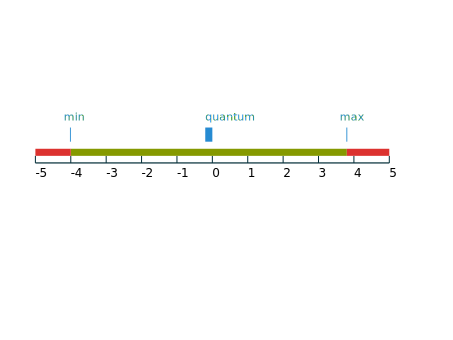
\includegraphics[width=\textwidth]{../../report/src/img/fixedPoint.pdf}
    \end{minipage}
\end{frame}

% {{{2 multimodem

\subsubsection{Multi modem support}
\begin{frame}
    \frametitle{Modem instance awareness}
    \begin{itemize}
        \item Voice processing algorithms
        \item Multiple modems for several phone carriers
        \item Big team effort of more than 200 patches
        \item Parameter-framework modem plugin
    \end{itemize}
\end{frame}

% {{{1 Opensourcing
\subsection{Open-sourcing the Parameter-framework}
\subsubsection{Context}
\begin{FrameWithSubSection}
    \begin{block}{Why open-sourcing this component?}
        \begin{itemize}
            \item Core component of Intel audio HAL
            \item Potential to become middleware standard
            \item Visibility
        \end{itemize}
    \end{block}
\end{FrameWithSubSection}

\subsubsection{Documentation}
\begin{frame}
    \frametitle{Newcomer documentation}
    \centering
    \begin{block}{Is the component ready for open-sourcing?}
        \begin{itemize}
            \item Code review and study
            \item Documentation for external contributors
            \item More than 450 lines of documentation
        \end{itemize}
    \end{block}
\end{frame}

\begin{frame}
    \frametitle{Newcomer documentation illustration}
    \centering
    \includegraphics[height=0.85\textheight]{../../report/src/img/tutos.pdf}
\end{frame}

\subsubsection{Branch sync process}
\begin{frame}
    \frametitle{Branch sync process}
    \begin{block}{How to open-source the component?}
        \begin{itemize}
            \item Ensure external contributions are of quality
            \item Avoid maintenance of 2 divergent code bases
            \item Ensure no confidential information is exposed
        \end{itemize}
    \end{block}
\end{frame}

\begin{frame}
    \frametitle{Branch sync process}
    \centering
    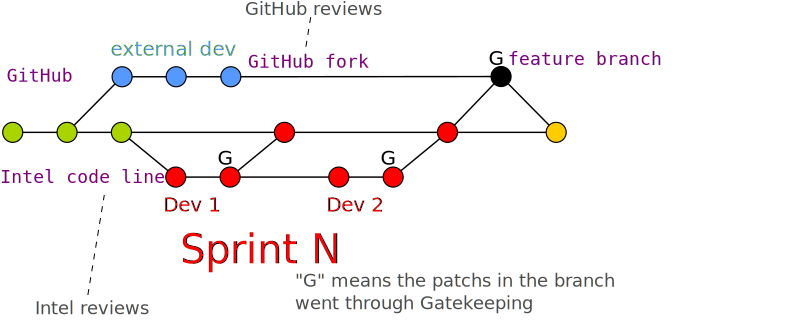
\includegraphics[width=\textwidth]{../../report/src/img/branches-process.pdf}
\end{frame}

\subsubsection{Open-sources projects}
\begin{frame}
    \frametitle{Projects which are open-source}
    \begin{block}{01org}
        \begin{itemize}
            \item \href{https://01.org/}{Intel Open Source Technology Center}
            \item \href{https://github.com/orgs/01org/teams/01-org-parameter-framework-owners}{GitHub organisation}
        \end{itemize}
   \end{block}
    \begin{block}{Projects on GitHub}
        \begin{itemize}
            \item Parameter-framework \href{https://github.com/01org/parameter-framework}{core}
            \item Parameter-framework \href{https://github.com/01org/parameter-framework-plugins-alsa}{ALSA plugin}
            \item Parameter-framework \href{https://github.com/01org/parameter-framework-plugins-filesystem}{filesystem plugin}
            \item Parameter-framework \href{https://github.com/01org/parameter-framework/wiki}{wiki}
            \item Parameter-framework \href{https://github.com/01org/parameter-framework-samples}{sample files}
        \end{itemize}
    \end{block}
\end{frame}

\begin{frame}
    \frametitle{GitHub top contributors}
    \centering
    \includegraphics[width=\textwidth]{../../report/src/img/statsGitHub.png}
\end{frame}


\chapter{Conclusion}
\section{subsect}
\subsection{subsub}
Hello, world.
Lorem ipsum dolar

AAAA bscdde

\subsection{}

\section{Global conclusion}


\end{document}
